\section{Conclusion}

\subsection{Technique}
\begin{frame}
    \frametitle{Conclusion Technique}

    \begin{figure}[H]
        \centering
        \begin{minipage}{.5\textwidth}
            \centering
            \begin{itemize}
                \item Finalisation de la programmation
                \item Expérience acquise grâce aux TPs
                \item La SAE est une matière complète, intéressante et enrichissante
            \end{itemize} 
        \end{minipage}%
        \begin{minipage}{.5\textwidth}
            \centering
            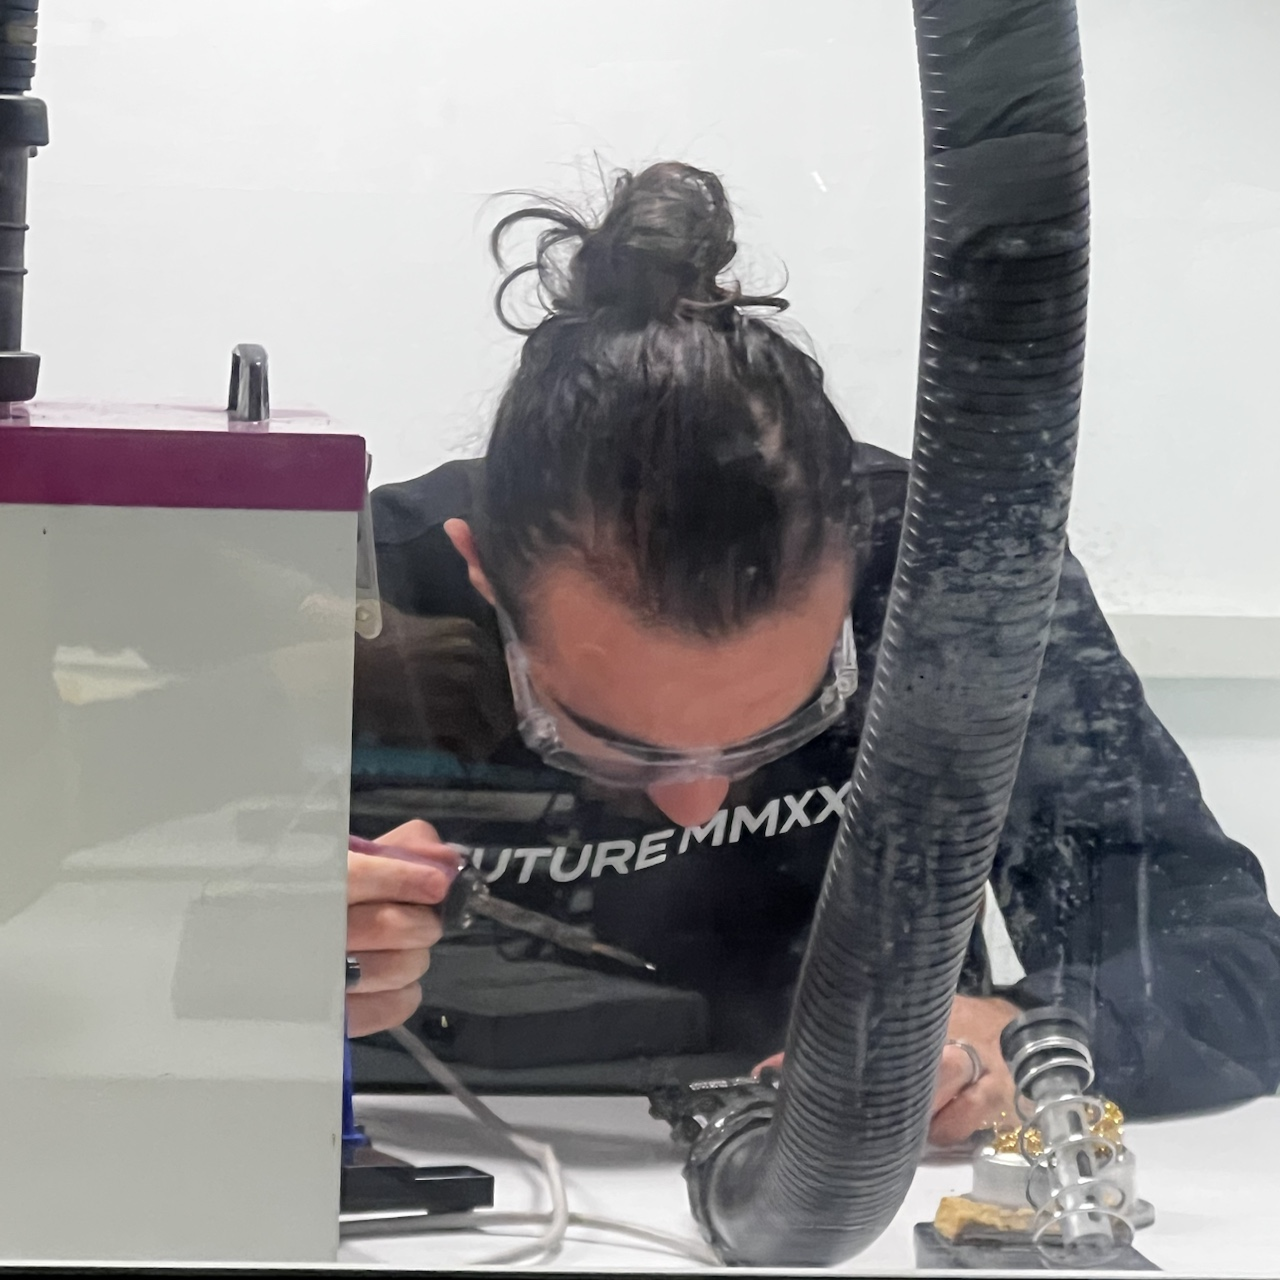
\includegraphics[width=.7\linewidth]{Images/fun.png}
            \caption{Le fun en personne}
            \label{fig:fun}
        \end{minipage}%
    \end{figure}
    
\footer{\hfill\insertframenumber/\inserttotalframenumber}
\end{frame}

\subsection{Humaine}
\begin{frame}{Organisation}
    \begin{figure}[H]
        \centering
        \begin{minipage}{.5\textwidth}
            \centering
            \begin{itemize}
                \item Permet de stocker des fichiers ainsi que toutes les versions de celui-ci
                \item Permet la gestion de projet grâce à un board de type "Trello"
                \item Permet de nous habituer à des standards utilisés en entreprise (git)
            \end{itemize} 
        \end{minipage}%
        \begin{minipage}{.5\textwidth}
            \centering
            
\includegraphics[width=.3\linewidth]{Images/github.png}
            \caption{GitHub}
            \label{fig:fun}
        \end{minipage}%
    \end{figure}
\end{frame}
\begin{frame}
    \frametitle{Conclusion humaine - OBS}
    \begin{figure}[H]
            \centering
            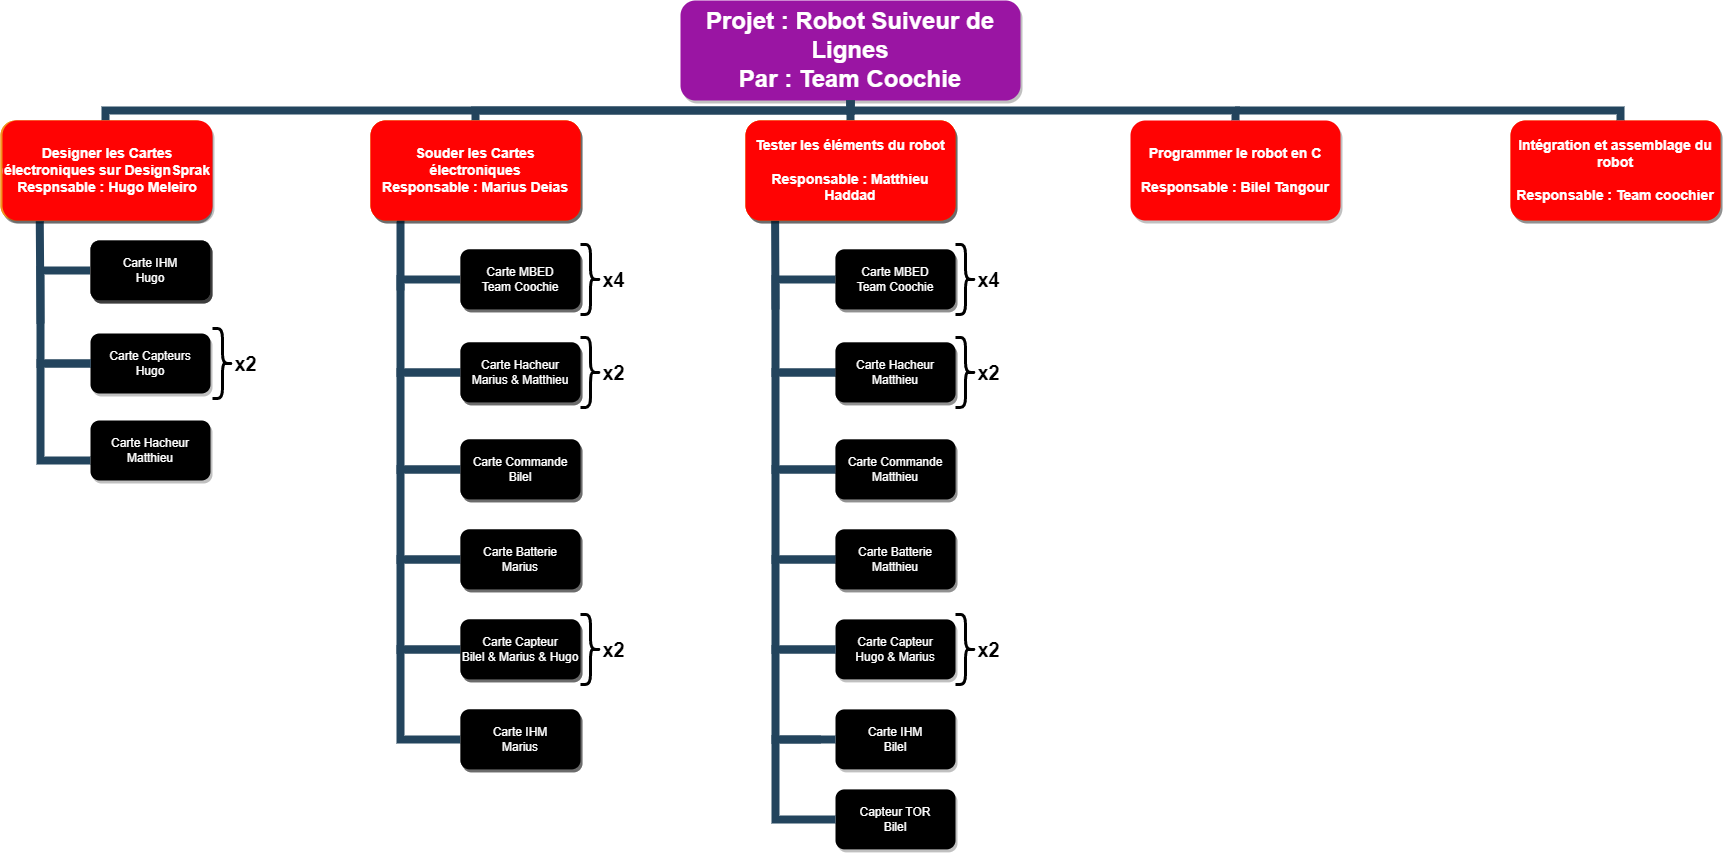
\includegraphics[width=0.8\linewidth]{Images/OBS.drawio.png}
    \end{figure}

\footer{\hfill\insertframenumber/\inserttotalframenumber}
\end{frame}